\documentclass{beamer}

% TODO (GM): Styling!
\usetheme{Copenhagen}
\setbeamertemplate{headline}{}

\usepackage{tikz}
\usepackage{pgfplots}
\usepackage{amsmath}
\usepackage{mathtools}
\usepackage[ngerman]{babel}

\usepackage{relsize}
\usepackage{algorithm}
\usepackage{algorithmic}
\usepackage{xcolor}
\usepackage{todonotes}

\presetkeys{todonotes}{inline}{}

\usetikzlibrary{overlay-beamer-styles}
\usetikzlibrary{arrows.meta,calc}

% -- BEGIN SECTION TOKENS AND CUSTOM COMMANDS --

\newcommand{\sectionstart}[1]{
    \section{#1}
    \begin{frame}
        \centering
        \huge{#1}
    \end{frame}
}

\newcommand{\R}{\ensuremath{\mathbb{R}}}
\newcommand{\Rn}{\ensuremath{\mathbb{R}^n}}
\newcommand{\Rnn}{\ensuremath{\mathbb{R}^{n \times n}}}
\newcommand{\Rd}{\ensuremath{\mathbb{R}^d}}

\newcommand{\Ltwo}{\ensuremath{{L^2(\Omega)}}}
\newcommand{\Hone}{\ensuremath{{H^1(\Omega)}}}
\newcommand{\Honez}{\ensuremath{{H^1_0(\Omega)}}}
\newcommand{\Hdual}{\ensuremath{{H^{-1}(\Omega)}}}

\newcommand{\mA}{\ensuremath{\mathcal{A}}}
\newcommand{\mAh}{\ensuremath{\mathcal{\tilde{A}}}}
\newcommand{\mI}{\ensuremath{\mathcal{I}}}
\renewcommand{\thealgorithm}{}

% -- END SECTION TOKENS AND CUSTOM COMMANDS --

% -- BEGIN SECTION SLIDES --

\title[]{Die Inverse Iteration für Eigenwertprobleme mit Eigenvektor-Nichtlinearitäten}
\author{Max Grübmeyer}
\date{11. Juli 2025}

\begin{document}
    \begin{frame}
        \titlepage
    \end{frame}

    \begin{frame}
        \frametitle{Gliederung}
        \tableofcontents[hideallsubsections]
    \end{frame}

    \sectionstart{Das Problem}

    \begin{frame}
        \frametitle{\insertsection}
        \begin{block}{Das Gross-Pitaevskii Energiefunktional}
            \centering
            $E(v) \coloneq \frac{1}{2} \mathlarger{\int}_{\Omega} \mathsmaller{\frac{1}{2}\vert \nabla v \vert ^2 + V \vert v \vert ^2 + \frac{\beta}{2}\vert v \vert ^4} \,dx$
        \end{block}

        \pause
        \bigskip

        \begin{itemize}
            \item $\Omega \subseteq \Rd$ beschränktes und konvexes Gebiet mit $d = 1,2,3$
                \pause
            \item $V \in L^\infty(\Omega)$ mit $V(x) \geq 0 $ für fast alle $x \in \Omega$
                \pause
            \item $\beta \geq 0$
        \end{itemize}

        \pause
        \bigskip

        \centering
        Gesucht $\underset{u \in H^1_0(\Omega)}{\mathrm{argmin}}\;E(u)$ mit $\Vert u \Vert_\Ltwo = 1$
    \end{frame}

    \begin{frame}
        \frametitle{Eine Alternative Formulierung}

        Wir suchen:
        \begin{align*}
            \mAh_u(u,\cdot) = \lambda(u,\cdot)_\Ltwo = 
            \lambda \mI u
        \end{align*}

        mit $\mAh_u: \Honez \rightarrow \Hdual$.

        \pause
        \bigskip

        \begin{block}{}
            Standardlösungstheorie für PDEs gibt uns
            \begin{align*}
                0 < \lambda_1 < \lambda_2 \leq \lambda_3 \leq ... \rightarrow \infty
            \end{align*}
        \end{block}
    \end{frame}

    \sectionstart{Die Inverse Iteration}

    \begin{frame}
        \frametitle{\insertsection}

        \begin{algorithm}[H]
            \caption{Inverse Iteration}
            \begin{algorithmic}[1]
                \STATE $u^0 \in \Honez$
                \FOR{$n=0$ to $Konvergenz$}
                \STATE $u^{n+1} = \frac
                {\mA_{u^n}^{-1} u^n}
                {\Vert \mA_{u^n}^{-1} u^n \Vert}$
                \ENDFOR
            \end{algorithmic}
        \end{algorithm}

        \pause

        Sei in unserem Fall $\mA_v^{-1} = \mAh_v^{-1}\mI$.
    \end{frame}

    \sectionstart{Ein erstes Konvergenzresultat}

    \begin{frame}
        \frametitle{{\insertsection} - Ostrowskis Theorem}
        \begin{block}{Ostrowskis Theorem}
            Sei $u \in \Honez$ und $\phi: \Honez \rightarrow \Honez$ mit Fréchet-Ableitung $\phi'(u)$ an der Stelle $u$.
            Hat diese Spektralradius $\rho(\phi'(u)) < 1$,
            dann existiert offene $H^1$ Umgebung $S$ von $u$, sodass die Fixpunktiteration
            \begin{align*}
                u^{n+1} = \phi(u^n)
            \end{align*}
            für alle $u^0 \in S$ gegen $u$ konvergiert.
        \end{block}

        \pause

        Genauer gilt dann: Für jedes $\varepsilon > 0$ existiert eine offene
        Umgebung $S_\varepsilon$ von $u$ und eine Konstante $C_\varepsilon > 0$:
        \begin{align*}
            \Vert u^n - u \Vert_\Hone \leq C_\varepsilon \vert \rho + \varepsilon \vert^n \Vert u^0 - u \Vert_\Hone\;\; \forall u^0 \in S_\varepsilon, n \geq 1
        \end{align*}
    \end{frame}

    \begin{frame}
        \frametitle{Spektralradius der Fréchet-Ableitung}
        \begin{block}{Abschätzung des Spektralradius}
            Es gilt:
            \begin{center}
                $\rho = \underset{i}{\mathrm{sup}} \vert \mu_i \vert
                \leq (1 - \delta) \frac{\lambda_1}{\lambda_2} < 1$
            \end{center}
            für ein $\delta \in (0,1)$.
        \end{block}

        \bigskip

        Somit garantiert uns Ostrowski's Theorem lokale Konvergenz.
    \end{frame}

    \sectionstart{Globale Konvergenz}

    \begin{frame}
        \frametitle{Eine Differentialgleichung}

        \begin{block}{Die Differentialgleichung}
            Betrachte
            \begin{align*}
                z'(t) = -z(t) + \gamma(z(t))\mA_{z(t)}^{-1}z(t)
            \end{align*}
            mit $\gamma(z) = (\mA_z^{-1} z, z)_\Ltwo^{-1}$.
        \end{block}

        \pause
        \medskip

        Man kann zeigen:
        \begin{align*}
            \frac{1}{2}\frac{d}{dt}\Vert z(t) \Vert^2 = 0
        \end{align*}

        \pause
        \medskip

        und
        \begin{align*}
            \frac{d}{dt}E(z(t)) \leq 0
        \end{align*}
    \end{frame}

    \begin{frame}
        \frametitle{Diskretisierung der Differentialgleichung}

        Für $z'(t^n) \approx \frac{z^{n+1} - z^{n}}{\tau_n}$:

        \pause

        \begin{align*}
            \frac{z^{n+1} - z^{n}}{\tau_n} = -z^n + \gamma(z^n)\mA_{z^n}^{-1}z^n
        \end{align*}

        \pause

        beziehungsweise

        \begin{align*}
            z^{n+1} = (1 - \tau_n)z^n + \tau_n \gamma(z^n) \mA_{z^n}^{-1}z^n
        \end{align*}
    \end{frame}

    \begin{frame}
        \frametitle{\insertsection}
        \begin{algorithm}[H]
            \caption{Gedämpfte Inverse Iteration}
            \begin{algorithmic}[1]
                \STATE $u^0 \in \Honez$
                \FOR{$n=0$ to $Konvergenz$}
                \STATE $u^{n+1} = \frac
                {(1-\tau_n)u^n + \tau_n\gamma(u^n)\mA_{u^n}^{-1} u^n}
                {\Vert(1-\tau_n)u^n + \tau_n\gamma(u^n)\mA_{u^n}^{-1} u^n\Vert}$
                \ENDFOR
            \end{algorithmic}
        \end{algorithm}
        \bigskip

        mit $\gamma(v) = (\mA_v^{-1} v, v)_\Ltwo^{-1}$
    \end{frame}

    \begin{frame}
        \frametitle{Theorem über die Globale Konvergenz}
        \begin{block}{Theorem über die Globale Konvergenz}
            Es exisitiert ein $\tau_{crit} \in (0,2)$, sodass die gedämpfte Inverse
            Iteration mit jeder Folge $(\tau_n)_{n \in \mathbb{N}}$, die
            \begin{align*}
                0 < \tau_n < \tau_{crit}
            \end{align*}
            erfüllt für alle Startwerte $u^0 \in \Honez$ mit $\Vert u^0 \Vert = 1$
            und $u^0 > 0$ konvergiert.


        \end{block}

        Insbesondere gilt dies für $\tau_{crit} \coloneq 2(1 + \frac{\lambda_1}{\lambda_2})^{-1} \in (1, 2)$.
    \end{frame}

    \begin{frame}
        \frametitle{Wahl des Dämpfungsparameters}

        \begin{block}{Wahl des Dämpfungsparameters}
            Wähle Dämpfungsparameter $\tau_n \in (0,2)$ mithilfe von Linensuchverfahren
            \begin{align*}
                \tau_n = \mathrm{arg min}
                    \mathlarger{\mathlarger{\mathlarger{\{}}}
                    E(\frac{(1 - \tau_n)u^n + \tau_n\gamma(u^n)\mA_{u^n}^{-1}(u^n)}
                    {\Vert(1 - \tau_n)u^n + \tau_n\gamma(u^n)\mA_{u^n}^{-1}(u^n)\Vert})
                    \mathlarger{\mathlarger{\mathlarger{\}}}}
            \end{align*}

            Wobei $E$ das Gross-Pitaevskii Energiefunktional ist.
        \end{block}
    \end{frame}


    \sectionstart{Numerische Simulation}

    \begin{frame}
        \frametitle{{\insertsection} - Setup}

        Betrachte
        \begin{align*}
            A(v) = L_N + M_V + \tilde{A}(v)
        \end{align*}

        \pause
        \bigskip

        Mit
        \begin{itemize}
            \item $L_N$ der diskretisierte Laplace
                \pause
            \item $M_V$ das Potential
                \pause
            \item $\tilde{A}(v) = \frac{1}{h^2}\beta diag(\vert v \vert)^2$ die Nichtlinearität
        \end{itemize}

        \pause
        \bigskip

        Gesucht Lösungen der Form $A(v)v = \lambda v$ mit minimalem $\lambda$
    \end{frame}

    \begin{frame}
        \frametitle{\insertsection}
        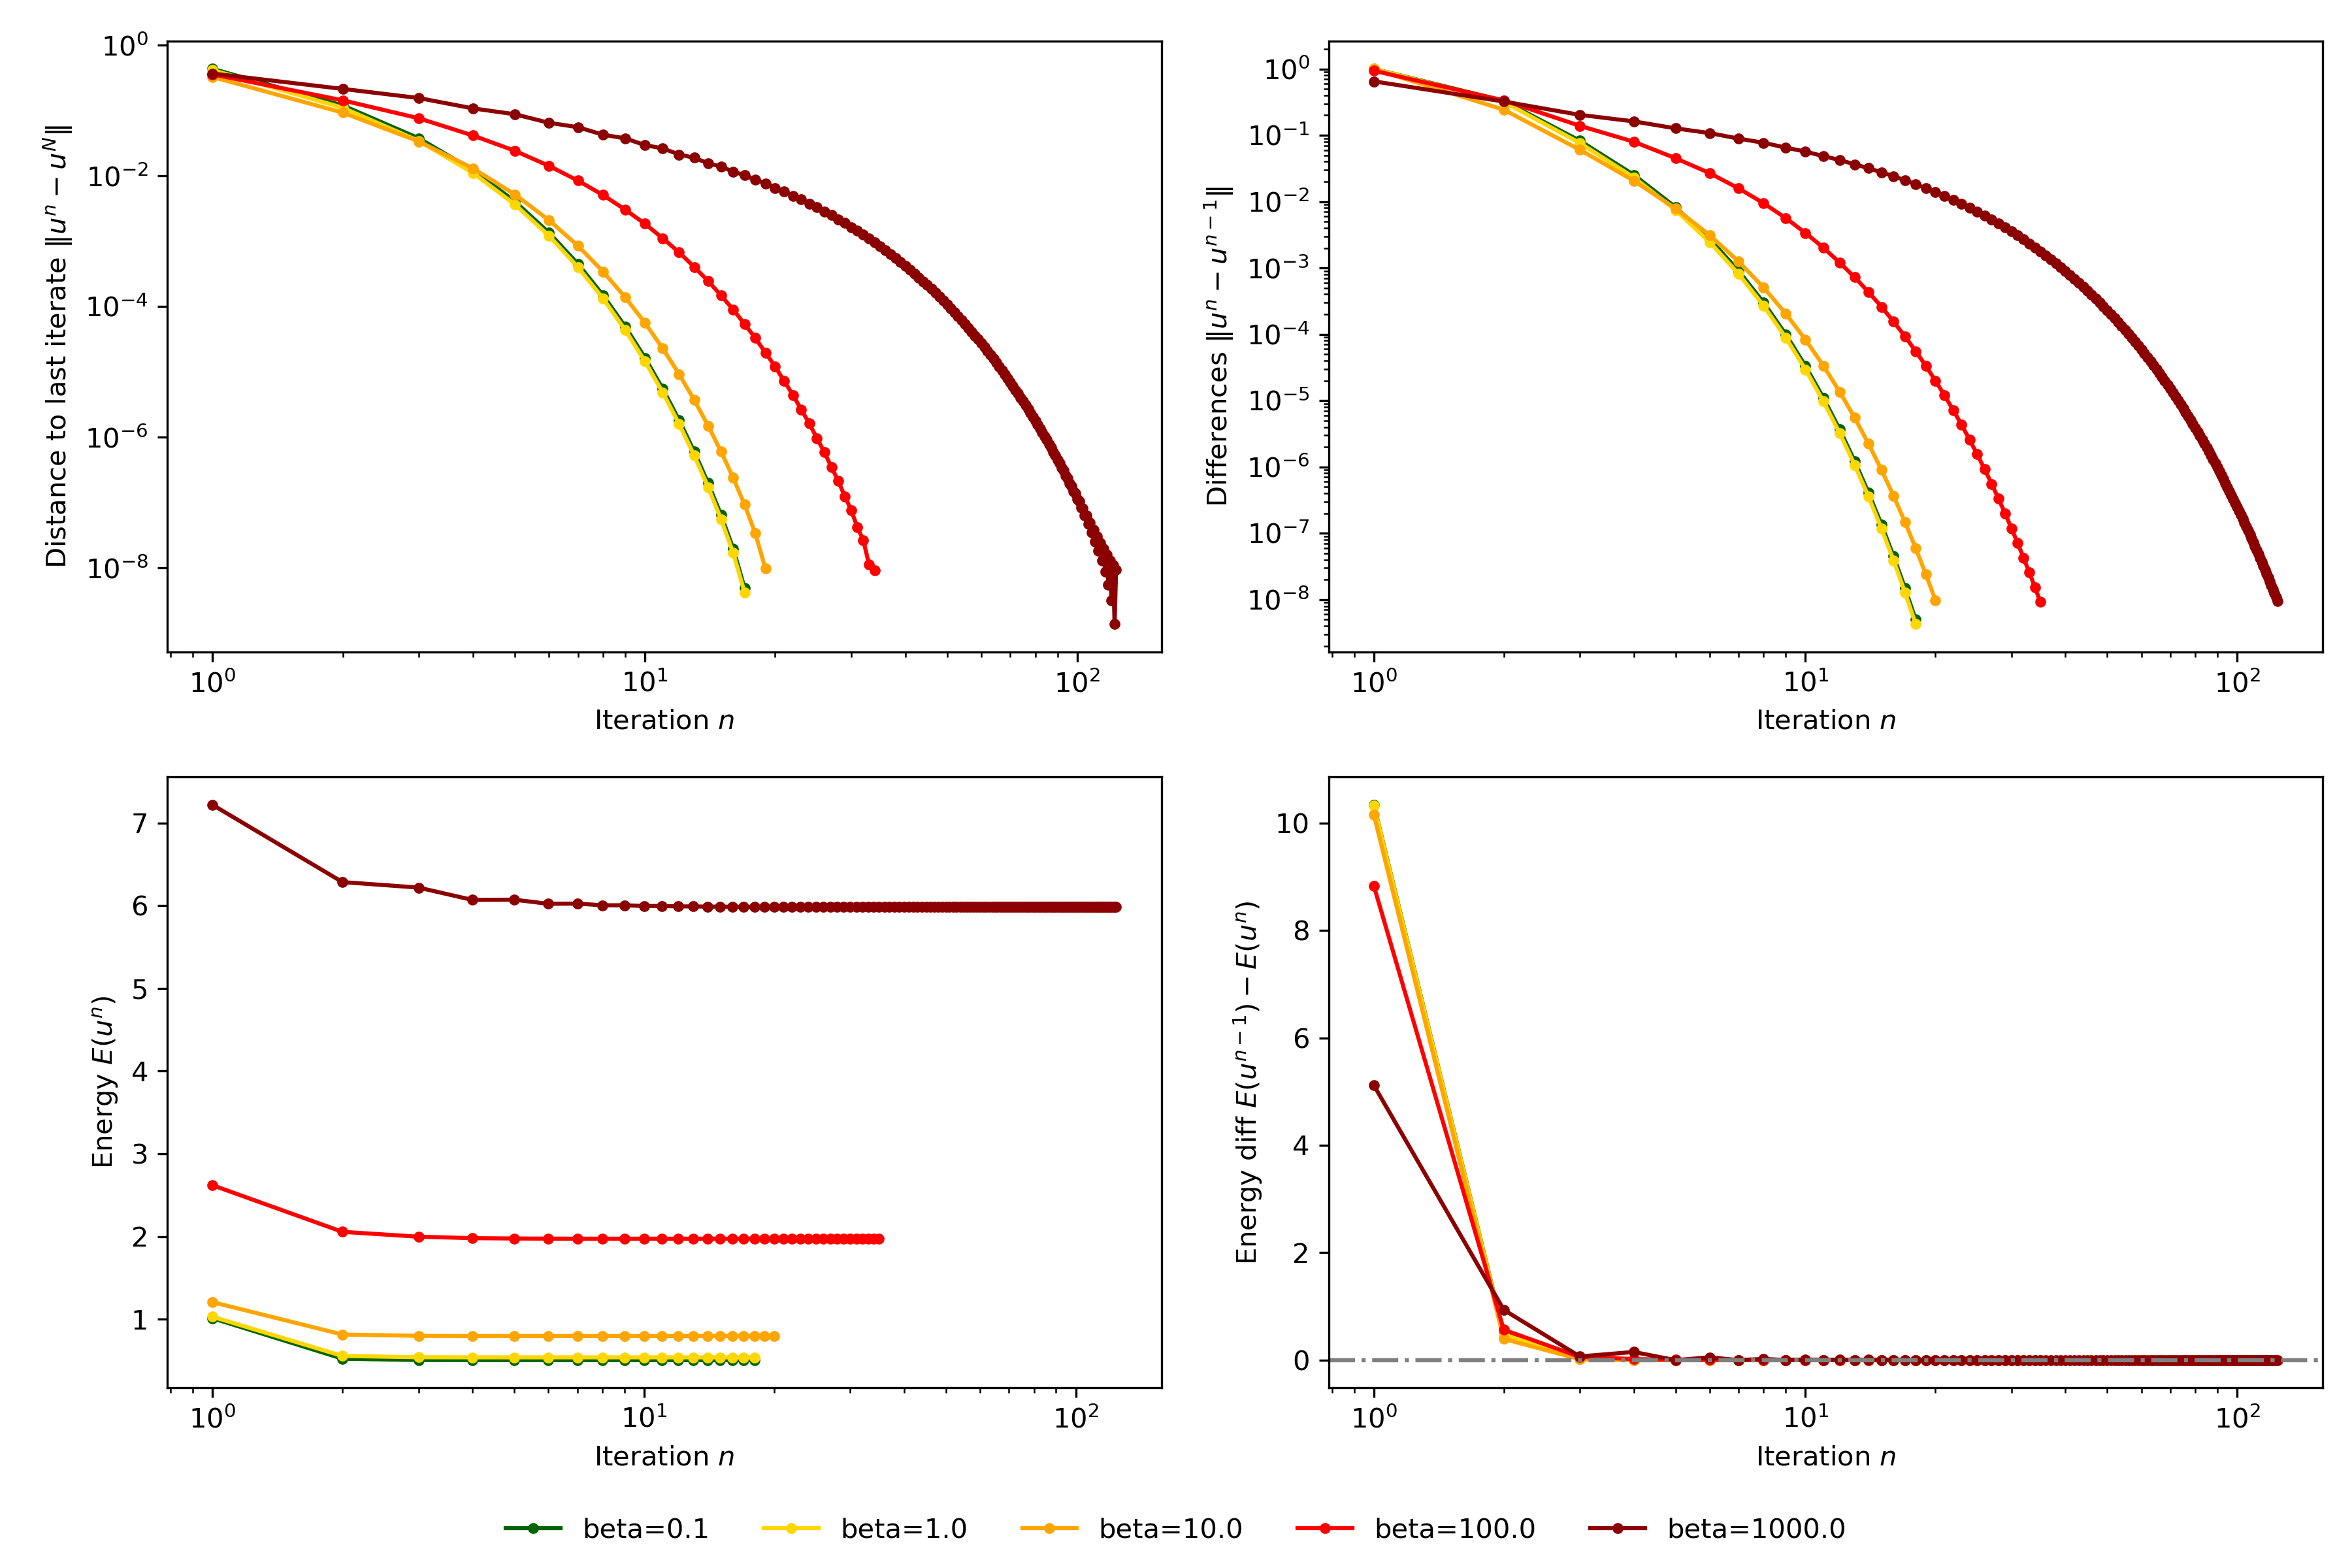
\includegraphics[width=\textwidth]{../img/gpe-inverse-iteration.png}
    \end{frame}

    \begin{frame}
        \frametitle{\insertsection}
		\centering
        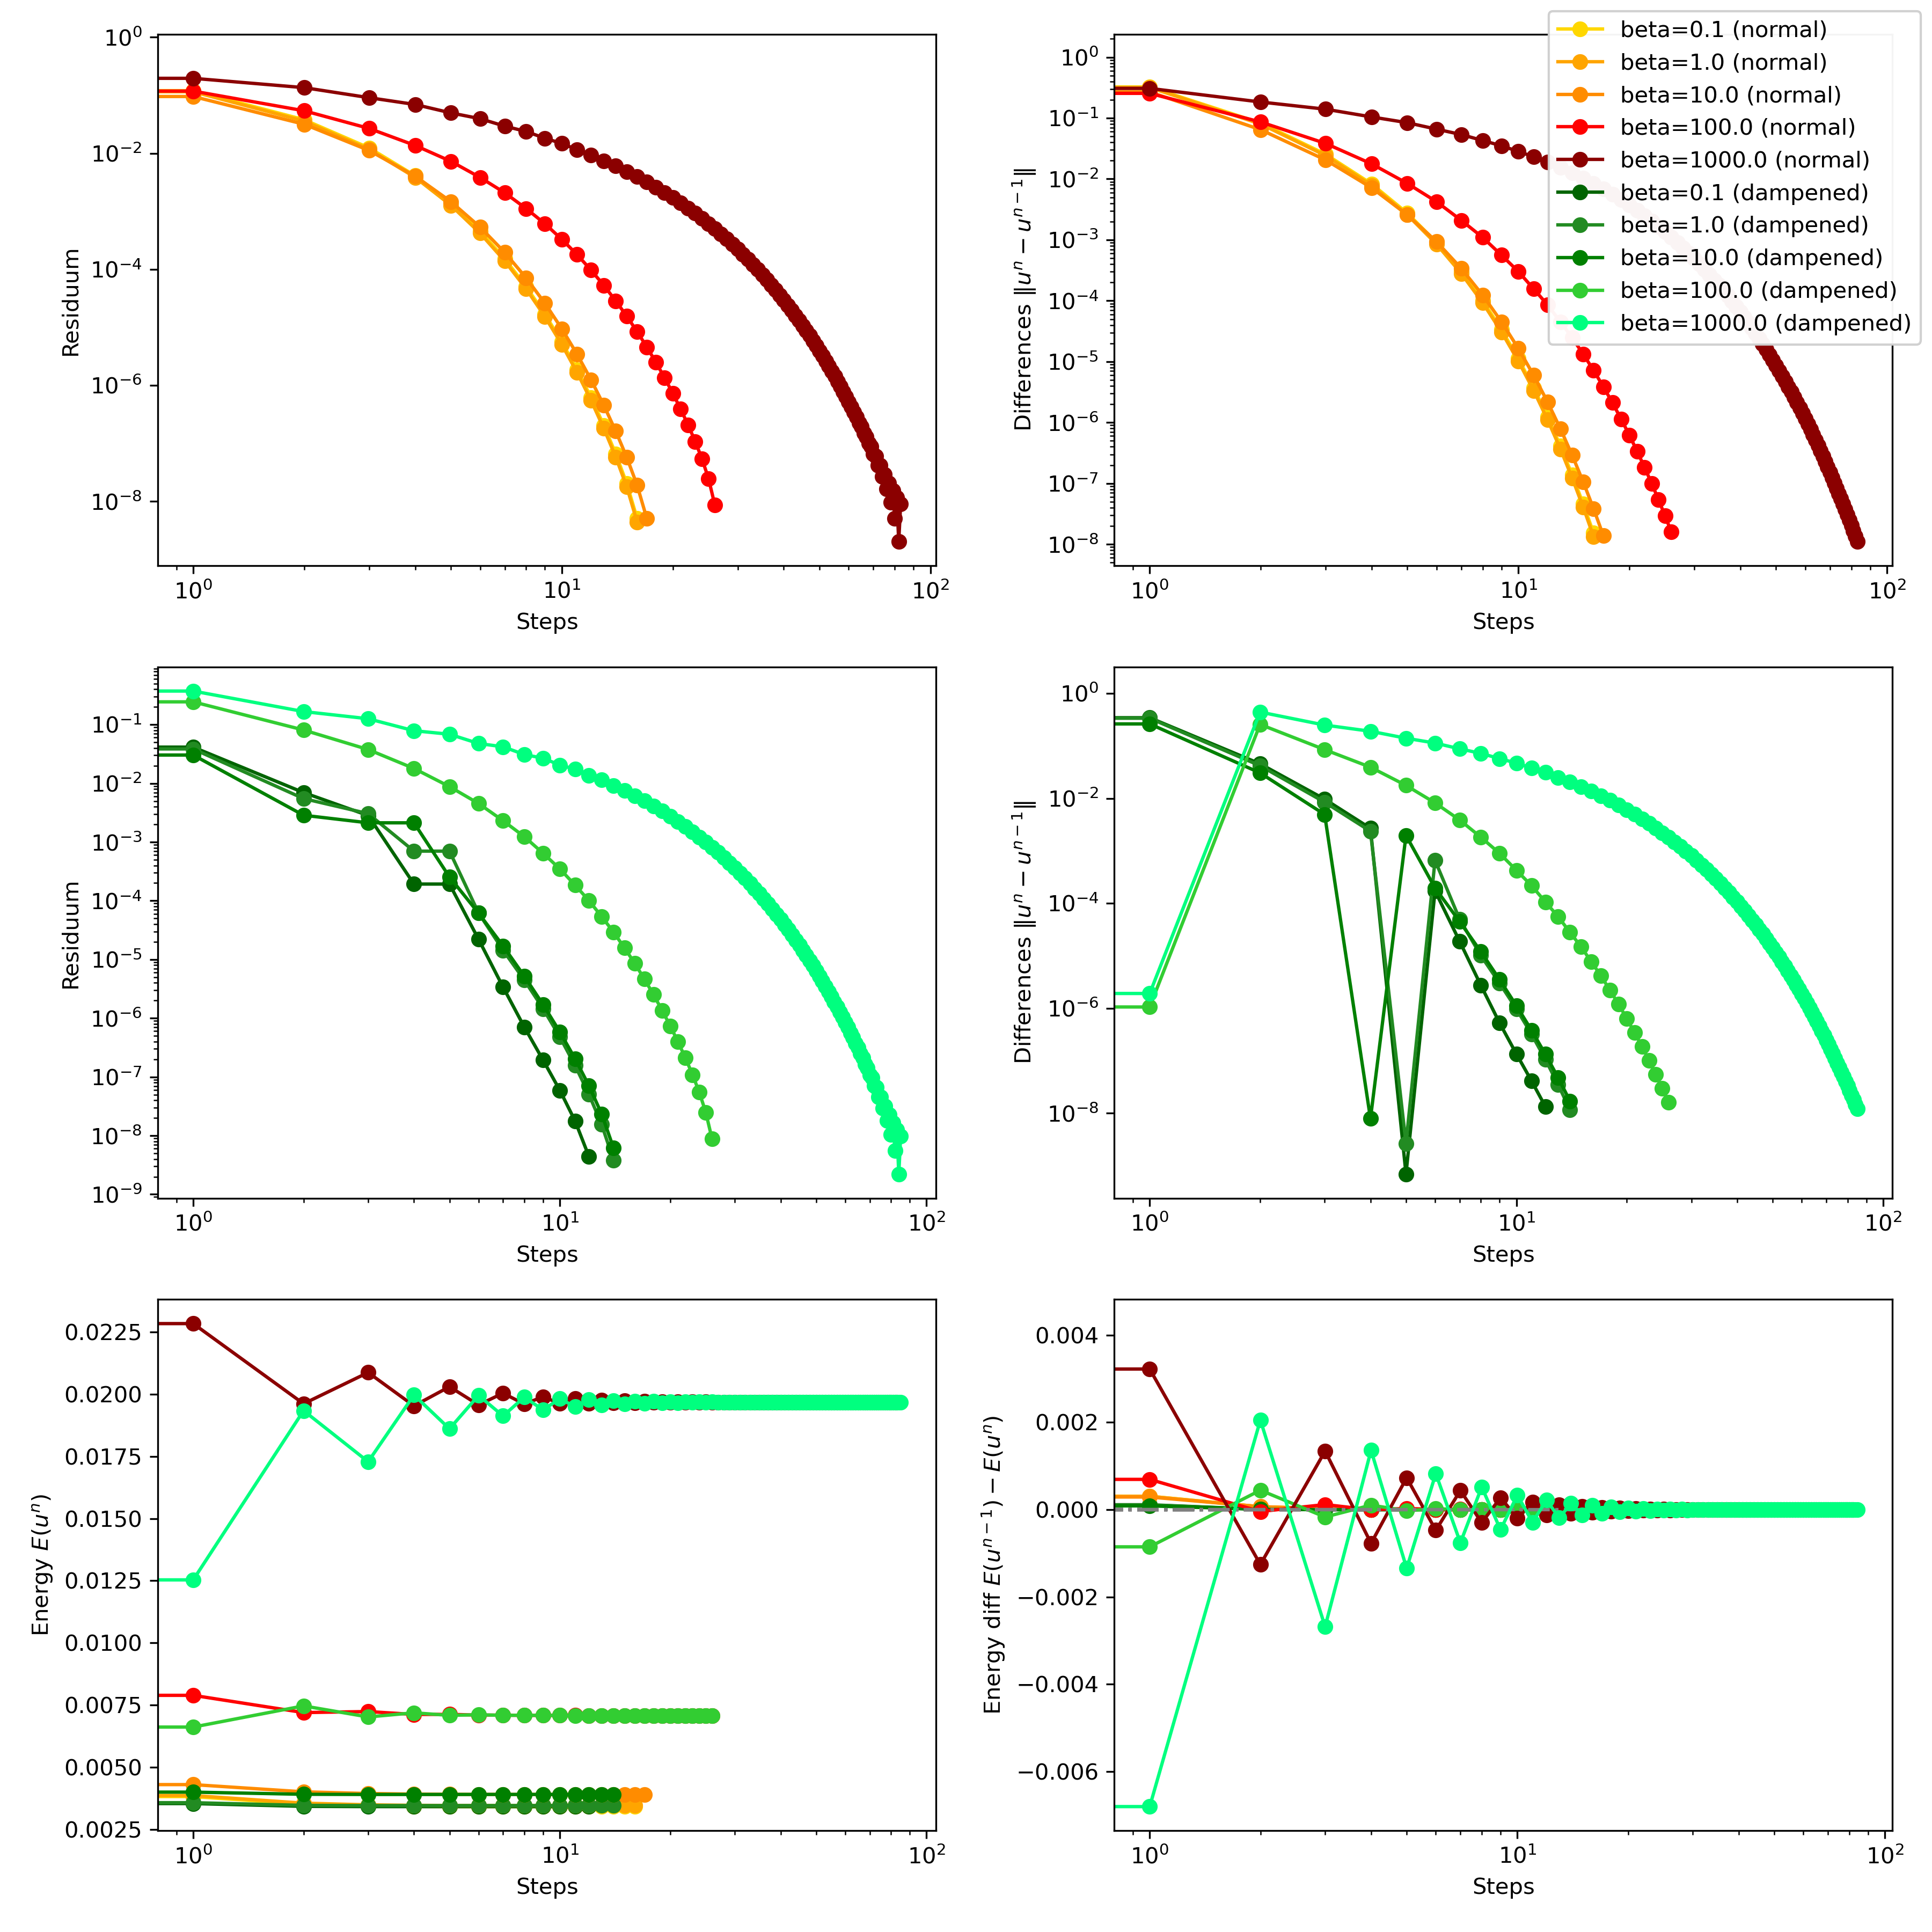
\includegraphics[height=0.85\textheight]{../img/gpe-inverse-iteration-comparision.png}
    \end{frame}
\end{document}

% -- END SECTION SLIDES --
